\chapter{Cuantizaci'on del Campo Electromagn'etico libre}

Despu'es de todo el desarrollo hecho para la cadena lineal, que era un modelo
unidimensional escalar, estamos en (mejores) condiciones de abordar la
cuantizaci'on del campo electromagn'etico.

Un primer paso para la cuantizaci'on es identificar las variables de campo. Como
veremos, en el caso del campo electromagn'etico esto no es trivial...

\section{Teor'ia cl'asica: Ecuaciones de Maxwell}

Sabemos que las ecuaciones de Maxwell son las ecuaciones que determinan
el comportamiento del campo electromagn'etico cl'asico. 'Estas se
dividen en dos grupos: las inhomog'eneas\footnote{Las leyes de Gauss y
la ley de Amp'ere-Maxwell.} que conectan los campos con sus fuentes: 
\begin{eqnarray}
\overrightarrow{\nabla}\cdot\overrightarrow{D}  =4\pi \rho\qquad
&\longleftrightarrow&\qquad\partial_{i}D_{i}=4\pi\rho ,\label{Ley de Gauss}\\
\overrightarrow{\nabla}\times\overrightarrow{H}  = \overrightarrow{j}
+\frac{1}{c}\frac{\partial\overrightarrow{D}}{\partial
t}\qquad&\longleftrightarrow&
\qquad\epsilon_{ijk}\partial_{j}H_{k}=\frac{4\pi}{c}j_{i}+\frac{1}{c}\frac{
\partial D_{i}}{\partial
t} ,\label{Ley de Ampere-Maxwell}
\end{eqnarray}
y las ecuaciones homog'eneas\footnote{Ley de Faraday y Ley de Biot-Savart.}, que
nos entregan relaciones que ligan al campo el'ectrico y magn'etico, y
condiciones que 'estos deben cumplir:
\begin{eqnarray}
\overrightarrow{\nabla}\times\overrightarrow{E}+\frac{1}{c}\frac{
\partial\overrightarrow
{B}}{\partial t}  = 0\qquad&\longleftrightarrow&\qquad\epsilon_{ijk}
\partial_{j}E_{k}+\frac{1}{c}\frac{\partial B_{i}}{\partial t}=0 ,\label{Ley de
Faraday}\\
\overrightarrow{\nabla}\cdot\overrightarrow{B}  = 0\qquad&\longleftrightarrow&
\qquad\partial_{i}B_{i}=0 .\label{Ley de Biot-Savart}
\end{eqnarray}
Por 'ultimo, tenemos las relaciones constitutivas, que contienen la informaci'on
sobre las propiedades del medio electromagn'etico considerado. En el vac'io,
estas son:
\begin{eqnarray}
\overrightarrow{D}  = \overrightarrow{E}\qquad
&\longleftrightarrow&\qquad D_{i}=E_{i} ,\label{ecuacion-Constitutiva-1}
\\
\overrightarrow{B}  = \overrightarrow{H}\qquad&\longleftrightarrow&
\qquad B_{i}=H_{i} .\label{ecuacion-Constitutiva-2}
\end{eqnarray}
Note que aqu'i hemos escrito las ecuaciones de Maxwell usando el sistema
gaussiano de unidades (c.g.s.), que es el que se presta m'as convenientemente
para nuestros fines.

En total, tenemos que las ecuaciones de Maxwell constituyen ocho ecuaciones
diferenciales \textit{de primer orden} que describen la evoluci'on de los
campos.

Que las ecuaciones de Maxwell sean de primer orden dificulta la descripci'on
lagrangeana del campo electromagn'etico, ya que, en general, un lagrangiano que
depende de los campos y sus primeras derivadas suministra \textit{ecuaciones de
movimiento de segundo orden} en los campos. M'as precisamente, no es posible
encontrar un lagrangeano dependiendo de $\vec{E}$, $\vec{B}$ y sus primeras
derivadas, que implique las ecuaciones de Maxwell como correspondientes
ecuaciones de Euler-Lagrange.

Sin embargo, es posible escribir las ecuaciones de Maxwell como ecuaciones
diferenciales de segundo orden si se introducen los campos auxiliares llamados
\textit{potenciales electromagn'eticos}: uno vectorial $A_{i}$ y el otro escalar
$\varphi$, tal que satisfagan identicamente las ecuaciones homog'eneas
(\ref{Ley de Faraday}) y (\ref{Ley de Biot-Savart}). Esto se consigue, como es
sabido, si
\begin{eqnarray}
B_{i} & = &\epsilon_{ijk}\partial_{j}A_{k}\label{Ai} ,\\
E_{i} & = &-\partial_{i}\varphi-\frac{1}{c}\partial_{t}A_{i} .\label{Phi}
\end{eqnarray}

Estas ecuaciones definen los campos el'ectrico y magn'etico en
funci'on de los potenciales electromagn'eticos.

Pero existe un ``problema" con los potenciales introducidos anteriormente: ellos
no son 'unicos. Esto se puede verificar efectuando siguiente cambio:
\begin{eqnarray}
A_{i}\qquad & \rightarrow\qquad A'_{i}=A_{i}+\partial_{i}\chi ,\label{Ai de
Gauge}\\
\varphi\qquad & \rightarrow\qquad\varphi'=\varphi-\frac{1}{c}\partial_{t}\chi
,\label{Phi de Gauge}
\end{eqnarray}
llamado \textit{transformaci'on de gauge}. Los nuevos $A'_{i}$ y $\varphi'$, que
dependen de los antiguos y de una funci'on $\chi=\chi\left( \vec{x},t\right)$,
tambi'en satisfacen las ecuaciones (\ref{Ai}) y  (\ref{Phi}), y por lo tanto las
ecuaciones de Maxwell homogeneas.

Por lo tanto, los potenciales poseen informaci'on redundante. Esto puede ser un
problema grave para la cuantizaci'on, puesto que al trabajar con los potenciales
electromagn'eticos estamos introduciendo grados de libertar superfluos en la
teor'ia. Por otro lado, la \textit{libertad de gauge} nos permite escoger
potenciales particulares que sean 'utiles para simplificar muchos c'alculos, sin
alterar la f'isica del sistema.

Usando las ecuaciones constitutivas e introduciendo (\ref{Ai}) y (\ref{Phi}) en
(\ref{Ley de Ampere-Maxwell}), obtenemos:
\begin{eqnarray}
\epsilon_{ijk}\partial_{j}\left( \epsilon_{klm}\partial
_{l}A_{m}\right) & = &\frac{4\pi}{c} j_{i}+\frac{1}{c}\partial_{t}\left(
-\partial_{i}\varphi-\frac{1}{c}\partial_{t}A_{i}\right) \nonumber\\
 &=&\frac{4\pi}{c}
j_{i}-\frac{1}{c}\partial_{t}\partial_{i}\varphi-\frac{1}{c^2}\partial_{t}
\partial_{t}A_{i} .
\end{eqnarray}
De este modo, podemos escribir
\begin{eqnarray}
\left( \delta_{il}\delta_{jm}-\delta_{im}\delta_{jl}\right) \partial
_{j}\partial_{l}A_{m}+\frac{1}{c}\partial_{i}\partial_{t}\varphi+\frac{1}{c^2}
\partial_{t}^{2}A_{i} & = &\frac{4\pi}{c} j_{i}\\
\partial_{j}\partial_{i}A_{j}-\partial_{j}\partial_{j}A_{i}+\frac{1}{c}\partial_
{i}\partial_{t}\varphi+\frac{1}{c^{2}}\partial_{t}^{2}A_{i} &=&\frac{4\pi}{c}
j_{i} \\
\frac{1}{c^{2}}\partial_{t}^{2}A_{i}-\partial_{j}\partial_{j}A_{i}+\partial_{i}
\left\{ \partial_{j}A_{j}+\frac{1}{c}\partial_{t}\varphi\right\} & =
&\frac{4\pi}{c} j_{i} \\
\left( \frac{1}{c^{2}}\partial_{t}^{2}-\partial_{j}\partial_{j}\right)
A_{i}+\partial_{i}\left\{
\partial_{j}A_{j}+\frac{1}{c}\partial_{t}\varphi\right\} & = &\frac{4\pi}{c}
j_{i}\\
\square A_{i}+\partial_{i}\left\{
\partial_{j}A_{j}+\frac{1}{c}\partial_{t}\varphi\right\} & = &\frac{4\pi}{c}
j_{i}, \label{ecuacion1}
\end{eqnarray}
Por otro lado, (\ref{Phi}) en (\ref{Ley de Gauss}) suministra:
\begin{eqnarray}
\partial_{i}\left( -\partial_{i}\varphi-\frac{1}{c}\partial_{t}A_{i}\right) & =
&4\pi \rho ,\\
\partial_{i}\partial_{i}\varphi+\frac{1}{c}\partial_{i}\partial_{t}A_{i} & =
&-4\pi\rho ,\\
\partial_{i}\partial_{i}\varphi+\frac{1}{c}\partial_{t}\left\{
\partial_{i}A_{i}\right\} & =&-4\pi\rho.\label{ecuacion2}
\end{eqnarray}

Hemos obtenido as'i dos ecuaciones diferenciales inhomog'eneas \textit{de
segundo orden}, pero que siguen siendo complicadas de resolver debido a los
segundos t'erminos del lado izquierdo. Es ahora donde podemos hacer uso de
la libertad de gauge mencionada. Existen dos gauges \textit{com'unmente} usados:

\subsubsection{Gauge de Lorentz}
En este caso, se eligen potenciales que satisfagan\footnote{Esta condici'on
siempre se puede satisfacer aplicando una
transformaci'on de Gauge sobre los campos $A_{i}$ y $\varphi.$ Veamos;
supongamos que partimos de potenciales que no satisfacen el gauge de Lorentz
anterior:
\begin{equation}
\partial_{j}A_{j}+\frac{1}{c}\partial_{t}\varphi\neq0 .
\end{equation}

Ahora, aplicando la transformaci'on de gauge dada por (\ref{Ai de Gauge}) y
(\ref{Phi de Gauge}) donde los nuevos potenciales s'i satisfacen el gauge de
Lorentz, es decir:
\begin{eqnarray}
0&=&\partial_{j}A'_{j}+\frac{1}{c}\partial_{t}\varphi'\\
& = &\partial_{j}\left( A_{j}+\partial_{j}\chi\right)
+\frac{1}{c}\partial_{t}\left( \varphi-\frac{1}{c}\partial_{t}\chi\right) \\
& = &\partial_{j}A_{j}+\partial_{j}\partial_{j}\chi+\frac{1}{c}\partial
_{t}\varphi-\frac{1}{c^{2}}\partial_{t}\partial_{t}\chi \\
& = &-\left( \frac{1}{c^{2}}\partial_{t}^{2}-\partial_{j}\partial_{j}\right)
\chi+\partial_{j}A_{j}+\frac{1}{c}\partial_{t}\varphi ,
\end{eqnarray}
de modo que
\begin{equation}
\square\chi = \partial_{j}A_{j}+\frac{1}{c}\partial_{t}\varphi ,
\end{equation} 
lo que nos dice que la funci'on $\chi$ debe resolver una ecuaci'on de onda
inhomogenea, cuya soluci'on siempre existe (aunque no es 'unica).}
\begin{equation}
\partial_{j}A_{j}+\frac{1}{c}\partial_{t}\varphi=0\label{Gauge de Lorentz} .
\end{equation}
Usando el gauge de Lorentz, las ecuaciones para los potenciales
(\ref{ecuacion1}) y (\ref{ecuacion2}), se reducen a: 
\begin{equation}
\square A_{i}=\frac{4\pi}{c} j_{i},
\end{equation}
y
\begin{eqnarray}
\partial_{i}\partial_{i}\varphi+\frac{1}{c}\partial_{t}\left\{
-\frac{1}{c}\partial_{t}\varphi\right\} & = &-4\pi\rho ,\\
\partial_{i}\partial_{i}\varphi-\frac{1}{c^2}\partial_{t}\partial_{t}\varphi & =
&-4\pi \rho ,\\
\frac{1}{c^{2}}\partial_{t}^{2}\varphi-\partial_{i}\partial_{i}\varphi &
=&4\pi \rho , \\
\square\varphi & = &4\pi \rho,
\end{eqnarray}
que son las conocidas ecuaciones de onda inhomog'eneas.

\subsubsection{Gauge de Coulomb}
En este caso, se eligen potenciales que satisfagan\footnote{De igual manera,
esta condici'on siempre pueder ser satisfecha. Partiendo de potenciales que no
satisfacen el gauge de Coulomb:
\begin{equation}
\partial_{i}A_{i}\neq0 , 
\end{equation}
y luego aplicando la transformaci'on de Gauge de manera que los nuevos
potenciales s'i satisfagan (\ref{Gauge de Coulomb}), tenemos:
\begin{eqnarray}
\partial_{i}A'_{i} & = &0 ,\\
\partial_{i}\left( A_{i}+\partial_{i}\chi\right) & = &0 ,\\
\square\chi & = &-\partial_{i}A_{i},
\end{eqnarray}
lo que nos dice que resolviendo la ecuaci'on anterior, la funci'on $\chi$
siempre existe.}
\begin{equation}
\partial_{i}A_{i}=0\label{Gauge de Coulomb}.
\end{equation}
As'i, usando el gauge de Coulomb, obtendremos que las ecuaciones para
los potenciales se reducen a las ecuaciones diferenciales de segundo orden:
\begin{eqnarray}
\square A_{i}+\frac{1}{c}\partial_{i}\partial_{t}\varphi & = &\frac{4\pi}{c}
j_{i},\\
\partial_{i}\partial_{i}\varphi & = &-4\pi\rho.
\end{eqnarray}
Adem'as, es posible imponer la condici'on adicional $\varphi=0$ siempre
y cuando $j_{i}=0$ y $\rho=0$, es decir, en el vac'io. De esta
manera eliminamos el potencial escalar, mientras que $A_{i}$ debe satisfacer
la ecuaci'on de onda homog'enea
\begin{equation}
\square A_{i}=0,\label{ecuacion de Onda para Ai}
\end{equation}
y el gauge de Coulomb.

Adicionalmente, al usar el Gauge de Coulomb tendremos que los campos
el'ectrico y magn'etico estar'an completamente definidos una vez
conocido el potencial vectorial $A_{i},$ mediante
\begin{eqnarray}
E_{i} & = &-\frac{1}{c}\partial_{t}A_{i}\label{Ei(Ai)}, \\
B_{i} & = &\epsilon_{ijk}\partial_{j}A_{k}. \label{Bi(Ai)}
\end{eqnarray}
De esta forma hemos eliminado el potencial escalar $\varphi$: los campos $E_{i}$
y
$B_{i}$ s'olo dependen del potencial vectorial, que ser'a nuestra 'unica
variable de campo. 

\subsection{Soluci'on cl'asica para el campo de radiaci'on en el gauge de
Coulomb}

An'alogamente al caso del campo escalar unidimensional, es conveniente
considerar el campo dentro de una caja de volumen $V=L^{3}$, con condiciones de
borde peri'odicas. Con esto se logra discretizar los valores del vector de onda
$\vec{k}$:
\begin{equation}
\vec{k}=\left( k_{x},k_{y},k_{z}\right) =\frac{2\pi}{L}\left(
n_{1},n_{2},n_{3}\right), \label{kperm}
\end{equation}
con $n_{i}\in\mathbb{Z}$ . Por lo tanto, s'olo son posibles algunos modos
normales para el campo EM, correspondiendo a cada uno de los valores discretos
de $\vec{k}.$

Considerando esta discretizaci'on, podemos escribir una soluci'on general de
(\ref{ecuacion de Onda para Ai}) como:
\begin{equation}
\vec{A}(\vec{x},t)=\sum_{\vec{k}}\left\{\vec{A}_{\vec{k}}(t)e^{i\vec{k}\cdot\vec
{x}}+\vec{A}_{\vec{k}}^*(t)e^{-i\vec{k}\cdot\vec{x}}\right\} , \label{solA}
\end{equation} 
donde $A_k(t)=\tilde{A}_k e^{-i\omega_kt}$ y la suma sobre $\vec{k}$ se extiende
sobre todos los valores posibles (\ref{kperm}), y adem'as
\begin{equation}
\omega_k=c|\vec{k}|
\end{equation} 
Adicionalmente, para satisfacer el gauge de Coulomb, ver (\ref{Gauge de
Coulomb}), es necesario que 
\begin{equation}
\vec{k}\cdot\vec{A}_{\vec{k}}=0 ,
\end{equation} 
es decir, $\vec{A}_{\vec{k}}$ debe ser perpendicular al vector de onda $k$.
Decimos entonces que  $\vec{A}(x,t)$ est'a constituido por \textit{ondas
transversales}. Esta condici'on sobre $\vec{A}_{\vec{k}}$ reduce su n'umero de
posibles componentes independientes de 3 a 2. En otras palabras (y debido a la
linealidad de las ecuaciones de Maxwell), para cada vector de onda $\vec{k}$
dado, los posibles vectores $\vec{A}_{\vec{k}}$ permitidos forman un espacio
vectorial bidimensional. Por esto, siempre es posible escribir 
\begin{equation}
\vec{A}_{\vec{k}}=N_{\vec{k}}\sum_{\sigma=1}^2
\check{\varepsilon}_{\vec{k}\sigma} a_{\vec{k}\sigma},
\end{equation} 
donde hemos introducido un factor (a'un no definido) $N_{\vec{k}}$ por
conveniencia futura, $\check{\varepsilon}_{\vec{k}1}$ y
$\check{\varepsilon}_{\vec{k}2}$ son dos vectores unitarios ortogonales entre si
y con el vector de onda $\vec{k}=|k|\check{k}$ y donde $a_{\vec{k}\sigma}$
representan las
amplitudes de cada modo. M'as a'un, es conveniente elegir los vectores
$\check{\varepsilon}_{\vec{k}\sigma}$ de modo que, para cada $\vec{k}$, el trio 
$\left(
\check{\varepsilon}_{\vec{k}1},\check{\varepsilon}_{\vec{k}2},\vec{k}\right)
$ formen una base ortonormal derecha, es decir:
\begin{equation}
\check{\varepsilon}_{\vec{k}1}\times\check{\varepsilon}_{\vec{k}2}=\check{k},
\qquad 
\check{\varepsilon}_{\vec{k}2}\times\check{k}=\check{\varepsilon}_{\vec{k}1},
\qquad
\check{k}\times\check{\varepsilon}_{\vec{k}1}=\check{\varepsilon}_{\vec{k}2}.
\end{equation}
Como consecuencia, los vectores $\check{\varepsilon}_{\vec{k}\sigma}$ satisfacen
las siguientes propiedades:
\begin{eqnarray}
\check{\varepsilon}_{\vec{k}\sigma}\cdot\vec{k} & = &0,\\
\check{\varepsilon}_{\vec{k}\sigma}\cdot\check{\varepsilon}_{\vec{k}\sigma'} & =
&\delta_{\sigma\sigma'},\qquad\sigma=1,2,\\
\check{\varepsilon}_{(-\vec{k})\sigma} & = &-\left( -1\right)
^{\sigma}\check{\varepsilon}_{\vec{k}\sigma},
\end{eqnarray}
tal como se puede verificar de la figura.  
\begin{figure}[ht]
\begin{center}
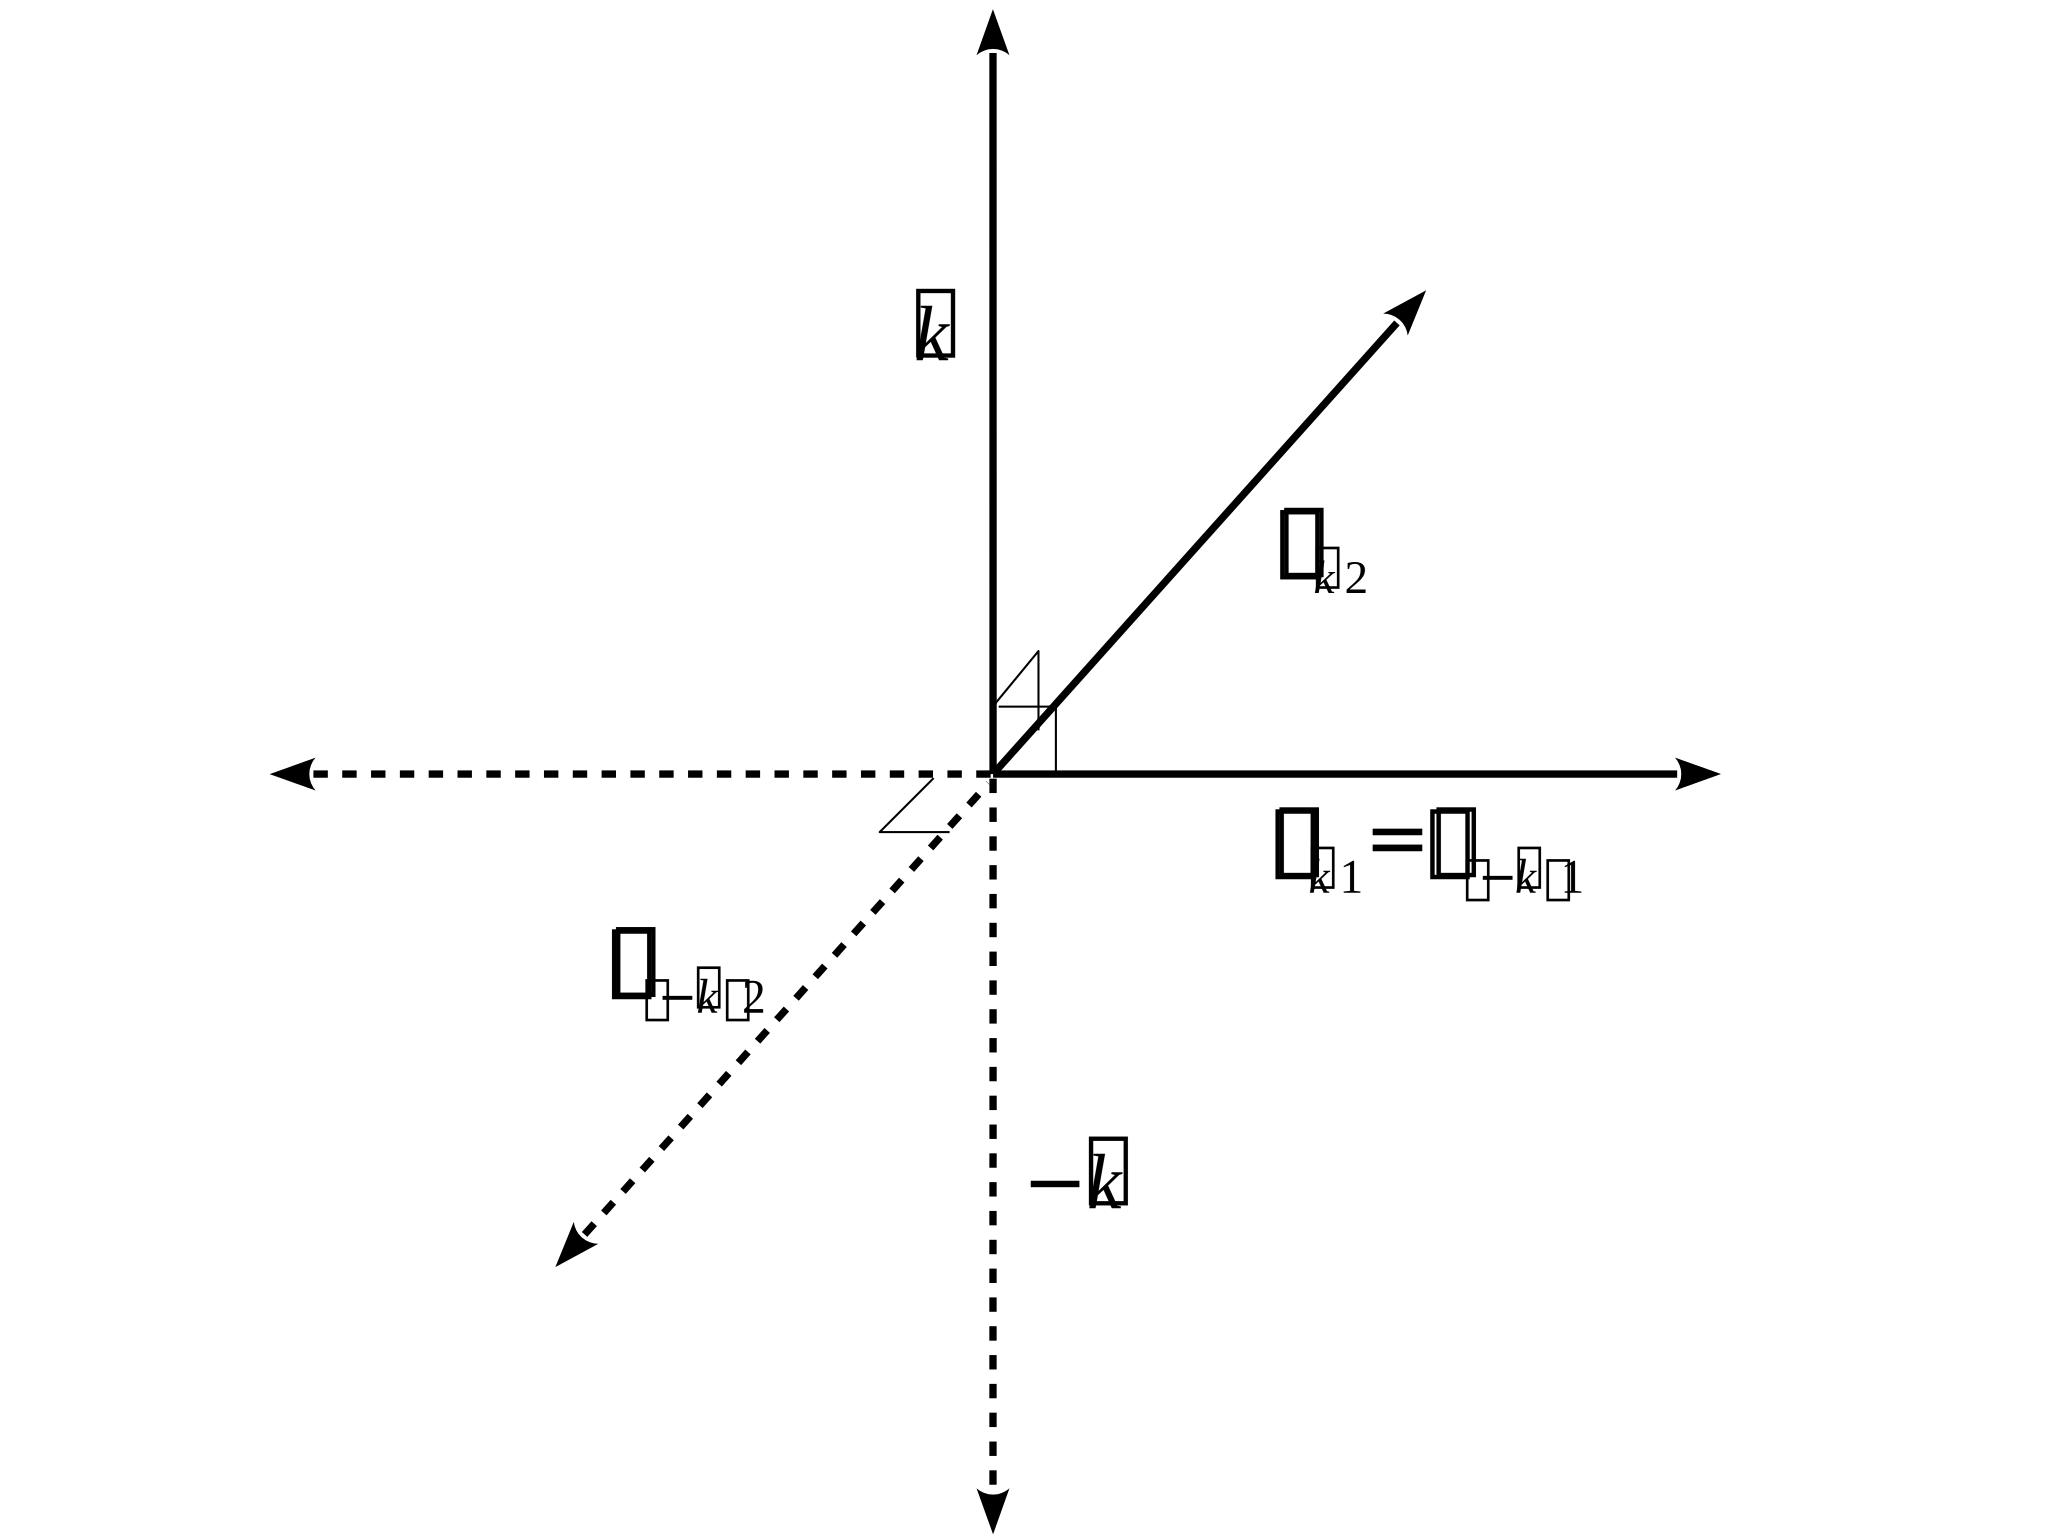
\includegraphics[height=4cm]{figs/fig-vec01.pdf}
\caption{Configuraci'on de los vectores $\check{\varepsilon}_{\vec{k}\sigma}$}
\label{figkep}
\end{center}
\end{figure}
En resumen, una soluci'on general de (\ref{ecuacion de Onda para Ai}) y
(\ref{Gauge de Coulomb}) puede escribirse como
\begin{equation}
\vec{A}(\vec{x},t)  =
\sum_{\sigma,\vec{k}}N_k\,\check{\varepsilon}_{\vec{k}\sigma}\left\{
a_{\vec{k}\sigma}(t)e^{i\vec{k}\cdot\vec{x}}+a_{\vec{k}\sigma}^*(t)e^{-i\vec{k}
\cdot\vec{x}}\right\} ,
\end{equation} 
es decir, como una superposici'on de ondas planas transversales, con dos modos
fundamentales independientes, uno para cada $\sigma$, denominadas
\textit{polarizaciones}. Es por esto que los vectores
$\check{\varepsilon}_{\vec{k}\sigma}$ son llamados \textit{vectores de
polarizaci'on}.

Como consecuencia, de (\ref{Ei(Ai)}) y (\ref{Bi(Ai)}) encontramos:
\begin{eqnarray}
\vec{E}(\vec{x},t)  & =
&\frac{i}{c}\sum_{\sigma,\vec{k}}N_k\,\check{\varepsilon}_{\vec{k}\sigma}\omega_
{k}\left\{
a_{\vec{k}\sigma}e^{i\vec{k}\cdot\vec{x}}-a_{\vec{k}\sigma}^*e^{-i\vec{k}
\cdot\vec{x}}\right\}, \\
\vec{B}(\vec{x},t) & = &i\sum_{\sigma,\vec{k}}N_k\left(
\vec{k}\times\check{\varepsilon}_{\vec{k}\sigma}\right) \left\{
a_{\vec{k}\sigma}e^{i\vec{k}\cdot\vec{x}}-a_{\vec{k}\sigma}^*e^{-i\vec{k}
\cdot\vec{x}}\right\} ,
\end{eqnarray}
de modo que tanto el campo el'ectrico como el magn'etico est'a constituido por
ondas transversales. Adem'as la energ'ia total y el momentum lineal total para
el campo electromagn'etico respectivamente son:
\begin{eqnarray}
H & = &\sum_{\sigma,\vec{k}}\frac{\omega_{k}^2}{8\pi c^2}N_k^2L^3\left(
a_{\vec{k}\sigma}^* a_{\vec{k}\sigma}+ a_{\vec{k}\sigma}
a_{\vec{k}\sigma}^*\right)  \\
\vec{P} & = &\sum_{\sigma,\vec{k}}\frac{\omega_{k}^2}{8\pi
c^2}N_k^2L^3\,\vec{k}\,a_{\vec{k}\sigma}^* a_{\vec{k}\sigma}
\end{eqnarray}


\subsection{Densidad lagrangeana, energ'ia y momentum lineal.}

Una densidad Lagrangeana que suministra las ecuaciones de Maxwell para los
$A_{i}$ es:%
\begin{equation}
{\cal L}=\frac{1}{8\pi}\left[ \frac{1}{c^{2}}\dot{A}_{i}\dot{A}_{i}-\left(
\partial_{i}A_{j}\right) \left(
\partial_{i}A_{j}\right)\right] , \label{Densidad Lagrangeana EM}
\end{equation}
donde el campo es sujeto adicionalmente a la condici'on adicional definida por
el gauge de Coulomb,
\begin{equation}
\partial_{i}A_{i}=0.
\end{equation} 
Usando la densidad lagrangeana (\ref{Densidad Lagrangeana EM}) podemos calcular:
\begin{equation}
\pi_{i}(\vec{x},t) = \frac{1}{4\pi c^{2}}\dot{A}_{i}=-\frac{1}{4\pi c}E_{i}
\label{DensidadMomentoCanonicoConjugado EM},
\end{equation}
\begin{eqnarray}
{\cal H}(\vec{x},t)& = &\frac{1}{4\pi c^{2}}\dot{A}_{i}\dot{A}_{i}-{\cal L}
\nonumber\\
& = &\frac{1}{4\pi c^{2}}\dot{A}_{i}\dot{A}_{i}-\frac{1}{8\pi c^{2}}\dot
{A}_{i}\dot{A}_{i}+\frac{1}{8\pi}\left( \partial_{i}A_{j}\right) \left(
\partial_{i}A_{j}\right) \nonumber\\
& = &\frac{1}{8\pi c^{2}}\dot{A}_{i}\dot{A}_{i}+\frac{1}{8\pi}\left(
\partial_{i}A_{j}\right) \left( \partial_{i}A_{j}\right) \nonumber\\
& = &\frac{1}{8\pi}\left\{ \frac{1}{c^{2}}\dot{A}_{i}\dot{A}_{i}+\left(
\partial_{i}A_{j}\right) \left( \partial_{i}A_{j}\right) \right\}
\label{Densidad Hamiltoniana EM}%
\end{eqnarray}
con lo que la energ'ia total es
\begin{equation}
H =\frac{1}{8\pi}\int dV \left\{ \frac{1}%
{c^{2}}\dot{A}_{i}\dot{A}_{i}+\left( \partial_{i}A_{j}\right) \left(
\partial_{i}A_{j}\right) \right\} \label{Energia del Campo EM1}%
\end{equation}
Usando la identidad
\begin{eqnarray}
B_{i}B_{i} & = &\epsilon_{ijk}\partial_{j}A_{k}\epsilon_{ilm}\partial_{l}%
A_{m}\\
& = &\left( \delta_{jl}\delta_{km}-\delta_{jm}\delta_{kl}\right) \left(
\partial_{j}A_{k}\right) \left( \partial_{l}A_{m}\right) \\
& = &\left( \partial_{j}A_{k}\right) \left( \partial_{j}A_{k}\right)
-\left( \partial_{j}A_{k}\right) \left( \partial_{k}A_{j}\right) \\
& = &\left( \partial_{j}A_{k}\right) \left( \partial_{j}A_{k}\right)
-\partial_{j}\left( A_{k}\partial_{k}A_{j}\right) +A_{k}\partial_{j}%
\partial_{k}A_{j}\\
& = &\left( \partial_{j}A_{k}\right) \left( \partial_{j}A_{k}\right)
-\partial_{j}\left( A_{k}\partial_{k}A_{j}\right)
+A_{k}\partial_{k}(\partial_{j}A_{j})\\
& = &\left( \partial_{j}A_{k}\right) \left( \partial_{j}A_{k}\right)
-\partial_{j}\left( A_{k}\partial_{k}A_{j}\right),
\end{eqnarray}
que es v'alida bajo el supuesto que el potencial vectorial satisface el gauge de
Coulomb, podemos escribir
\begin{eqnarray}
H & = &\frac{1}{8\pi}\int dV\left\{ \frac
{1}{c^{2}}\dot{A}_{i}\dot{A}_{i}+\left( \partial_{i}A_{j}\right) \left(
\partial_{i}A_{j}\right) \right\} \nonumber\\
& = &\frac{1}{8\pi}\int dV\left\{ \frac{1}{c^{2}}\dot{A}_{i}\dot{A}%
_{i}+B_{i}B_{i}+\partial_{j}\left( A_{k}\partial_{k}A_{j}\right) \right\}
\nonumber\\
& = &\frac{1}{8\pi}\int dV\left\{ \left(E^{2}+B^{2}\right) +\partial_{j}\left(
A_{k}\partial_{k}A_{j}\right) \right\} \nonumber\\
& = &\frac{1}{8\pi}\int dV\left( E^{2}+B^{2}\right) +\frac{1}{8\pi}\int
dV\partial_{j}\left( A_{k}%
\partial_{k}A_{j}\right) \nonumber\\
& = &\frac{1}{8\pi}\int_{V}dV\left( E^{2}+B^{2}\right)
+\frac{1}{8\pi}\oint_{\partial V}dS_{j}\,A_{k}\partial_{k}%
A_{j}\nonumber\\
& = &\frac{1}{8\pi}\int_{V}dV\left( E^{2}+B^{2}\right),\label{Energia del Campo
EM2}%
\end{eqnarray}
donde la integral de volumen $\oint_{\partial V}dS_{k}A_{k}\partial_{k}A_{j}$ se
anula debido a que asumimos el campo se anula suficientemente r'apido en el
infinito.

Por otro lado, para el momentum lineal total del sistema, obtenemos:
\begin{eqnarray}
p_{i}(\vec{x},t)& = &-\frac{1}{4\pi c^{2}}\dot{A}_{j}\partial_{i}A_{j}\\
& = &\frac{1}{4\pi c}\left\{ \left( \vec{E}\times\vec{B}\right) _{i}%
-\partial_{j}\left(\frac{1}{c} \dot{A}_{j}A_{i}\right) \right\}, \label{denpem}
\end{eqnarray}
ya que, en el gauge de Coulomb,
\begin{eqnarray}
\left( \vec{E}\times\vec{B}\right) _{i} & = &\epsilon_{ijk}E_{j}B_{k}\\
& = &\epsilon_{ijk}\left( -\frac{1}{c}\dot{A}_{j}\right) \left( \epsilon_{klm}%
\partial_{l}A_{m}\right) \\
& = &-\frac{1}{c}\epsilon_{ijk}\epsilon_{klm}\dot{A}_{j}\partial_{l}A_{m}\\
& = &-\frac{1}{c}\left( \delta_{il}\delta_{jm}-\delta_{im}\delta_{jl}\right)
\dot{A}%
_{j}\partial_{l}A_{m}\\
& =
&-\frac{1}{c}\dot{A}_{j}\partial_{i}A_{j}+\frac{1}{c}\dot{A}_{j}\partial_{j}A_{i
}\\
& = &-\frac{1}{c}\dot{A}_{j}\partial_{i}A_{j}+\frac{1}{c}\partial_{j}\left(
\dot{A}_{j}A_{i}\right)
-\frac{1}{c}A_{i}\partial_{j}\dot{A}_{j}\\
& = &-\frac{1}{c}\dot{A}_{j}\partial_{i}A_{j}+\frac{1}{c}\partial_{j}\left(
\dot{A}_{j}A_{i}\right)
-\frac{1}{c}A_{i}\partial_{t}\left( \partial_{j}A_{j}\right)\\
& = &-\frac{1}{c}\dot{A}_{j}\partial_{i}A_{j}+\frac{1}{c}\partial_{j}\left(
\dot{A}_{j}A_{i}\right).
\end{eqnarray}
Usando (\ref{denpem}), el momentum lineal total almacenado en el campo
electromagn'etico puede escribirse como
\begin{equation}
\vec{P}=\frac{1}{4\pi c}\int_{V}dV \vec{E}\times\vec{B} ,\label{Momentum Lineal
Total EM2}%
\end{equation} 
que corresponde al conocido vector de Pointing.


\section{Cuantizaci'on}

Dentro del gauge Coulomb y en el vac'io, donde podemos elegir $\phi=0$, lo
natural ser'ia considerar al potencial vectorial $A_i(\vec{x},t) $ como nuestra
variable de campo, de modo que su momento can'onico asociado ser'ia
\begin{equation}
\pi_i(\vec{x},t) =-\frac{1}{4\pi c}E_i(\vec{x},t).
\end{equation}
Para cuantizar el campo EM libre, debemos entonces promover estas variables de
campo a operadores que act'uan un espacio Hilbert, y luego conocer sus
relaciones de conmutaci'on.

Si consideramos a $A_i(\vec{x},t) $ como los campos independientes, entonces
esperar'iamos, de acuerdo al procedimiento de cuantizaci'on can'onico, que los
operadores de campo $\hat{A}_i(\vec{x},t)$ y $\hat{\pi}_i(\vec{x},t)$ satisfagan
las relaciones de conmutaci'on can'onicas
\begin{equation}
\left[\hat{A}_i(\vec{x}',t),\hat{\pi}_j(\vec{x},t)\right]
=i\hbar\,\delta_{ij}\,\delta(\vec{x}-\vec{x}') \hat{1}. \label{casicasi}
\end{equation}
Sin embargo, puede comprobarse r'apidamente que este conmutador es inconsistente
con el gauge de Coulomb
$\partial_i\hat{A}_{i}=\hat{0}$, ya que esta 'ultima condici'on implica
\begin{equation}
\partial_{j}'\left[ \hat{\pi}_i(\vec{x},t) ,\hat{A}_{j}(\vec{x}',t) \right] =
\left[ \hat{\pi}_i(\vec{x},t) ,\partial_{j}'\hat{A}_{j}(\vec{x}',t) \right] =0,
\end{equation}
pero, por otro lado, (\ref{casicasi}) requiere que
\begin{equation}
\partial_{j}'\left[ \hat{\pi}_i(\vec{x},t) ,\hat{A}_{j}(\vec{x}',t) \right]
=i\hbar\,\delta_{ij}\,\partial_{j}'\delta(\vec{x}-\vec{x}') \hat{1}\neq 0 .
\end{equation} 

Por lo tanto, no podemos usar las relaciones de conmutaci'on can'onicas para
cuantizar el campo electromagn'etico en el gauge de Coulomb.

Un camino para poder cuantizar el campo electromagn'etico de manera lo m'as
similar posible a la cuantizaci'on can'onica, es intentar modificar el lado
derecho de  (\ref{casicasi}) de modo que las nuevas relaciones de conmutaci'on
para los campos cu'anticos sean compatibles con el gauge de Coulomb. No es
dificil verificar\footnote{Usando $\nabla^2\frac{1}{\left| x_{k}-x'_{k}\right|
}=-4\pi\delta (\vec{x}-\vec{x}')$.}  que la modificaci'on requerida es 
\begin{equation}
\left[ \hat{A}_{i}(\vec{x},t) ,\hat{\pi}_{j}(\vec{x}',t) \right] =i\hbar\left\{
\delta_{ij}\delta (\vec{x}-\vec{x}')
+\frac{1}{4\pi}\partial_i\partial_j\frac{1}{\left| \vec{x}-\vec{x}'\right|
}\right\}
\hat{1}\label{Rel Conm Pi, A}
\end{equation}
Debido a que el nuevo t'ermino no se anula para $\vec{x}\neq\vec{x}'$, la
interpretaci'on estandar de la teor'ia cu'antica sugerir'ia que no es posible
medir simult'aneamente $\hat{A}_{i}(\vec{x},t)$ y $\hat{\pi}_{j}(\vec{x}',t)$ en
puntos distintos del espacio. Sin embargo, esto no representa necesariamente un
problema ya que $\hat{A}_{i}$ no es un observable (los observables son el campo
el'ectrico y el magn'etico). Podemos comprobar, por otra parte, que las nuevas
relaciones de conmutaci'on (\ref{casicasi}) implican relaciones de conmutaci'on
entre los campos el'ectricos y magn'eticos que no presentan este (aparente)
problema. En efecto, (\ref{casicasi}) implica
\begin{equation}
\left[\hat{B}_i(\vec{x},t),\hat{E}_j(\vec{x}',t)\right] =4\pi i\hbar
c\,\epsilon_{ijk}\partial_k\,\delta (\vec{x}-\vec{x}') \hat{1},
\end{equation} 
de modo que es posible medir simult'aneamente el campo el'ectrico y magn'etico
en puntos distintos del espacio. Sin embargo, estos campos no pueden
determinarse simult'aneamente con infinita precisi'on en el mismo punto del
espacio. Esto tiene como consecuencia que no puede existir un estado en el que
tanto $\vec{E}$ como $\vec{B}$ sean exactamente cero, lo que se manifiesta en
as'i llamadas, fluctuaciones del vac'io del campo electromagn'etico.

Finalmente, las relaciones 
\begin{eqnarray}
\left[\hat{A}_i(\vec{x},t),\hat{A}_j(\vec{x}',t)\right] &=&0,\\
\left[\hat{\pi}_i(\vec{x},t),\hat{\pi}_j(\vec{x}',t)\right] &=&0,
\end{eqnarray} 
completan las relaciones de conmutaci'on necesarias para la cuantizaci'on del
campo.



\subsection{Operadores de creaci'on y desctrucci'on}
An'alogamente al caso del campo escalar, puede mostrarse a partir de las
relaciones de conmutaci'on que los campos cu'anticos satisfacen las mismas
ecuaciones diferenciales que sus an'alogos cl'asicos.

Por lo tanto, podemos usar expansiones para los operadores de campo an'alogas a
aquellas del caso cl'asico, es decir,
\begin{eqnarray}
\hat{\vec{A}}(\vec{x},t)  &=&
\sum_{\vec{k},\sigma}N_k\,\check{\varepsilon}_{\vec{k}\sigma}\left\{
\hat{a}_{\vec{k}\sigma}(t)e^{i\vec{k}\cdot\vec{x}}+\hat{a}_{\vec{k}\sigma}
^\dagger (t)e^{-i\vec{k}\cdot\vec{x}}\right\} ,\\
\hat{\vec{E}}(\vec{x},t)  & =
&\frac{i}{c}\sum_{\vec{k},\sigma}N_k\,\check{\varepsilon}_{\vec{k}\sigma}\omega_
{k}\left\{
\hat{a}_{\vec{k}\sigma}e^{i\vec{k}\cdot\vec{x}}-\hat{a}_{\vec{k}\sigma}^\dagger
e^{-i\vec{k}\cdot\vec{x}}\right\}, \\
\hat{\vec{B}}(\vec{x},t) & = &i\sum_{\vec{k},\sigma}N_k\left(
\vec{k}\times\check{\varepsilon}_{\vec{k}\sigma}\right) \left\{
\hat{a}_{\vec{k}\sigma}e^{i\vec{k}\cdot\vec{x}}-\hat{a}_{\vec{k}\sigma}^\dagger
e^{-i\vec{k}\cdot\vec{x}}\right\} ,\\
\hat{H} & = &\sum_{\vec{k},\sigma}\frac{\omega_{k}^2}{4\pi c^2}N_k^2L^3\left(
\hat{a}_{\vec{k}\sigma}^\dagger \hat{a}_{\vec{k}\sigma}+ \hat{a}_{\vec{k}\sigma}
\hat{a}_{\vec{k}\sigma}^\dagger\right)  \\
\hat{\vec{P}} & = &\sum_{\vec{k},\sigma}\frac{\omega_{k}}{4\pi
c^2}N_k^2L^3\,\vec{k}\,\left( \hat{a}_{\vec{k}\sigma}^\dagger
\hat{a}_{\vec{k}\sigma}+ \hat{a}_{\vec{k}\sigma}
\hat{a}_{\vec{k}\sigma}^\dagger\right) .\\
\end{eqnarray}
De estas expresiones podemos obtener las relaciones inversas de los operadores
$\hat{a}$ y $\hat{a}^\dagger$ en funci'on de $\hat{A}_i$ y $\hat{\pi}_i$:
\begin{equation}
\hat{a}_{\vec{k}\sigma}=\frac{1}{2L^3N_k\omega_k}\int dV \left(\omega_{k}%
\hat{\vec{A}}+4\pi c^2 i \hat{\vec{\pi}}\right) \cdot
\check{\varepsilon}_{\vec{k}\sigma}e^{-i\vec{k}\cdot\vec{x}},
\end{equation}
y, como consecuencia,
\begin{equation}
\hat{a}^\dagger_{\vec{k}\sigma}=\frac{1}{2L^3N_k\omega_k}\int dV
\left(\omega_{k}%
\hat{\vec{A}}-4\pi c^2 i \hat{\vec{\pi}}\right) \cdot
\check{\varepsilon}_{\vec{k}\sigma}e^{i\vec{k}\cdot\vec{x}}%
\end{equation}
Con estas expresiones, podemos calcular los conmutadores de $\hat{a}$ y
$\hat{a}^\dagger$. Obtenemos:
\begin{eqnarray}
\left[ \hat{a}_{\vec{k}\sigma},\hat{a}_{\vec{k}'\sigma '}^{\dagger}\right]
&=&\frac{2\pi\hbar c^2}{L^3\omega_kN_k^2}\,\delta_{\sigma\sigma
'}\delta_{\vec{k},\vec{k}'}  , \label{aad}\\
\left[ \hat{a}_{\vec{k}\sigma},\hat{a}_{\vec{k}'\sigma '}\right] &=&0. 
\end{eqnarray}
En este momento, elegimos la constante $N_k$ de modo conveniente. Definimos
\begin{equation}
N_k=\sqrt{\frac{2\pi\hbar c^2}{L^3\omega_k}},
\end{equation} 
de modo que los operadores $\hat{a}$ y $\hat{a}^\dagger$ sean adimensionales y
satisfagan relaciones de conmutaci'on tipo operadores ``escalera" del oscilador
arm'onico.

En resumen los campos cu'anticos que describen el campo electromagn'etico en el
gauge de Coulomb son:
\begin{eqnarray}
\hat{\vec{A}}(\vec{x},t)  &=& \sqrt{\frac{2\pi\hbar
c^2}{L^3}}\sum_{\vec{k},\sigma}\frac{1}{\sqrt{\omega_k}}\check{\varepsilon}_{
\vec{k}\sigma}\left\{
\hat{a}_{\vec{k}\sigma}(t)e^{i\vec{k}\cdot\vec{x}}+\hat{a}_{\vec{k}\sigma}
^\dagger (t)e^{-i\vec{k}\cdot\vec{x}}\right\} , \label{Afi}\\
\hat{\vec{E}}(\vec{x},t)  & =
&i\sqrt{\frac{2\pi\hbar}{L^3}}\sum_{\vec{k},\sigma}\frac{1}{\sqrt{\omega_k}}
\check{\varepsilon}_{\vec{k}\sigma}\omega_{k}\left\{
\hat{a}_{\vec{k}\sigma}e^{i\vec{k}\cdot\vec{x}}-\hat{a}_{\vec{k}\sigma}^\dagger
e^{-i\vec{k}\cdot\vec{x}}\right\}, \\
\hat{\vec{B}}(\vec{x},t) & = &i\sqrt{\frac{2\pi\hbar
c^2}{L^3}}\sum_{\vec{k},\sigma}\frac{1}{\sqrt{\omega_k}}\left(
\vec{k}\times\check{\varepsilon}_{\vec{k}\sigma}\right) \left\{
\hat{a}_{\vec{k}\sigma}e^{i\vec{k}\cdot\vec{x}}-\hat{a}_{\vec{k}\sigma}^\dagger
e^{-i\vec{k}\cdot\vec{x}}\right\} ,\\
\hat{H} & = &\frac{\hbar}{2}\sum_{\vec{k},\sigma}\omega_k\left(
\hat{a}_{\vec{k}\sigma}^\dagger \hat{a}_{\vec{k}\sigma}+ \hat{a}_{\vec{k}\sigma}
\hat{a}_{\vec{k}\sigma}^\dagger\right)  \\
\hat{\vec{P}} & = &\frac{\hbar}{2}\sum_{\vec{k},\sigma}\vec{k}\,\left(
\hat{a}_{\vec{k}\sigma}^\dagger \hat{a}_{\vec{k}\sigma}+ \hat{a}_{\vec{k}\sigma}
\hat{a}_{\vec{k}\sigma}^\dagger\right) ,\\
\end{eqnarray}
y satisfacen las relaciones de conmutaci'on siguientes:
\begin{eqnarray}
\left[ \hat{a}_{\vec{k}\sigma},\hat{a}_{\vec{k}'\sigma '}^{\dagger}\right]
&=&\delta_{\sigma\sigma'}\delta_{\vec{k},\vec{k}'}  , \label{aadf}\\
\left[ \hat{a}_{\vec{k}\sigma},\hat{a}_{\vec{k}'\sigma '}\right] &=&0.
\label{aadf2}
\end{eqnarray}


\subsection{Vectores de Estado del Campo Electromagn'etico.}

Procedemos de manera an'aloga a como lo hicimos en el caso del campo escalar
(secci'on \ref{secints}). Usando las relaciones de conmutaci'on
(\ref{aadf})-(\ref{aadf2}) escribimos el operador energ'ia como
\begin{equation}
\hat{H}  = \hbar\sum_{\vec{k},\sigma}\,\omega_{k}\left\{
\hat{a}_{\vec{k,\sigma}}^{\dagger} \hat{a}_{\vec{k},\sigma} +\frac{1}{2}
\right\}.
\end{equation} 
En el caso del operador momentum, tendremos que
\begin{equation}
\hat{P}  = \hbar\sum_{\vec{k},\sigma}\, \vec{k}\left\{
\hat{a}_{\vec{k},\sigma}^{\dagger} \hat{a}_{\vec{k},\sigma} +\frac{1}{2}
\right\}=\hbar\sum_{\vec{k},\sigma}\,
\vec{k}\,\hat{a}_{\vec{k},\sigma}^{\dagger}\hat{a}_{\vec{k},\sigma}.
\end{equation} 
El ``operador n'umero", asociado a cada modo $(\vec{k},\sigma)$ con vector de
onda y polarizaci'on definidas, se define como:
\begin{equation}
\hat{N}_{\vec{k},\sigma}:=\hat{a}_{\vec{k},\sigma}^{\dagger}\hat{a}_{\vec{k},
\sigma} ,\label{defNa}
\end{equation}
de modo que los operadores Hamiltoniano y el momentum se escriben como:%
\begin{eqnarray}
\hat{H} & = &\hbar\sum_{\vec{k},\sigma}
\omega_{k}\hat{N}_{\vec{k},\sigma}+\frac{1}{2}\hbar\sum_{\vec{k},\sigma}
\omega_{k}  ,\\
\hat{P} & = &\hbar\sum_{\vec{k},\sigma} \vec{k}\,\hat{N}_{\vec{k},\sigma} .
\end{eqnarray}
Consecuentemente, encontramos que los conmutadores del operador n'umero con
$\hat{a}_{\vec{k},\sigma}$ y $\hat{a}_{\vec{k},\sigma}^{\dagger}$ son
\begin{eqnarray}
\left[ \hat{N}_{\vec{k},\sigma},\hat{a}_{\vec{k}',\sigma'}\right]
&=&-\delta_{k,k'}\delta_{\sigma,\sigma'}\,\hat{a}_{\vec{k},\sigma}, \\
\left[ \hat{N}_{\vec{k},\sigma},\hat{a}^{\dagger}_{\vec{k}',\sigma'}\right]
&=&\delta_{k,k'}\delta_{\sigma,\sigma'}\,\hat{a}^{\dagger}_{\vec{k},\sigma},
\end{eqnarray} 
de modo que
\begin{eqnarray}
\left[ \hat{H},\hat{a}_{\vec{k},\sigma}\right] &=&-\hbar\omega_k\,
\hat{a}_{\vec{k}}, \label{comha}\\
\left[ \hat{H},\hat{a}^{\dagger}_{\vec{k},\sigma}\right]
&=&\hbar\omega_k\,\hat{a}^{\dagger}_{\vec{k},\sigma},
\end{eqnarray} 
y
\begin{eqnarray}
\left[ \hat{P},\hat{a}_{\vec{k},\sigma}\right] &=&-\hbar \vec{k}\,
\hat{a}_{\vec{k},\sigma}, \\
\left[ \hat{P},\hat{a}^{\dagger}_{\vec{k},\sigma}\right] &=&\hbar \vec{k}\,
\hat{a}^{\dagger}_{\vec{k},\sigma} \label{compad}.
\end{eqnarray}
An'alogamente al caso escalar, estas propiedades implican que el espectro de
energ'ias y momenta del campo electromagn'etico cu'antico es discreto. Los
correspondientes cuantos de energ'ia y momentun son $h\omega_k$ y $\hbar
\vec{k}$, para un vector de onda $\vec{k}$ dado, respectivamente. El operador
$\hat{a}_{\vec{k},\sigma}$ (cuando se aplica a un estado dado) disminuye la
energ'ia y el momentum del estado del campo y es por esto interpretado como un
\textit{operador de destrucci'on de un cuanto de energ'ia y momentum del campo
electromagn'etico} (un ``fot'on"). An'alogamente,
$\hat{a}^{\dagger}_{\vec{k},\sigma}$ aumenta la energ'ia y el momentum del
estado del campo y es por esto interpretado como un \textit{operador de
creaci'on de un cuanto de energ'ia y momentum del campo electromagn'etico} (un
``fot'on"). 

La existencia de un estado de energ'ia m'inima, que denotaremos por
$\left|0\right>$, requiere que
\begin{equation}
\hat{a}_{\vec{k},\sigma}\left|0\right> =0, \qquad \forall\ \vec{k}, \forall \
\sigma .
\end{equation}
Este estado fundamental del campo cu'antico tiene momentum cero,
$\hat{P}\left|0\right> =0$, pero su energ'ia es infinita, con $E_0=
\frac{1}{2}\hbar\sum_{\vec{k},\sigma} \omega_{k} $.

Un estado de n'umero arbitrario puede entonces escribirse como
\begin{eqnarray}
\left| \dots,n_{\vec{k},\sigma},\dots,n_{\vec{k}',\sigma'},\dots\right>
&:=&\frac{1}{\sqrt{\cdots n_{\vec{k},\sigma}!\cdots
n_{\vec{k}',\sigma'}!\cdots}}\cdots \nonumber\\
&&\times\left( \hat{a}_{\vec{k},\sigma}^{\dagger}\right)
^{n_{\vec{k},\sigma}}\cdots\left( \hat{a}_{\vec{k}',\sigma'}^{\dagger}\right)
^{n_{\vec{k}',\sigma'}}\cdots\left| 0\right> ,
\end{eqnarray}
con $n_{\vec{k},\sigma}\in \mathbb{N}$, que interpretamos como un estado del
campo con $n_{\vec{k},\sigma}$ fotones cada una con energ'ia $\hbar\omega_{k}$
y momentum $\hbar \vec{k},$, $n_{\vec{k}',\sigma'}$ part'iculas con energ'ia y
momentum $\hbar\omega_{k'},$ $\hbar \vec{k}'$, etc, ya que
\begin{eqnarray}
\hat{H}\left| \dots,n_{\vec{k},\sigma},\dots,n_{\vec{k}',\sigma'},\dots\right>
&=& \left( E_0+n_{\vec{k},\sigma} \hbar\omega_k +n_{\vec{k}',\sigma'}
\hbar\omega_{k'}+\cdots\right) \nonumber\\
&&\times \left| \dots,n_{\vec{k},\sigma},\dots,n_{\vec{k}',\sigma'},\dots\right>
,\\
\hat{\vec{P}}\left|
\dots,n_{\vec{k},\sigma},\dots,n_{\vec{k}',\sigma'},\dots\right> &=& 
\left(n_{\vec{k},\sigma} \hbar \vec{k} +n_{\vec{k}',\sigma'} \hbar
\vec{k'}+\cdots\right) \nonumber\\
&&\times\left| \dots,n_{\vec{k},\sigma},\dots,n_{\vec{k}',\sigma'},\dots\right>
.
\end{eqnarray}

La acci'on de los operadores de creaci'on y destrucci'on sobre un estado $\left|
\dots,n_{\vec{k},\sigma},\dots\right>$ de n'umero del campo viene dada por
\begin{eqnarray}
\hat{a}_{\vec{k},\sigma}^{\dagger}\left| \dots,n_{\vec{k},\sigma},\dots\right> &
= &\sqrt{n_{\vec{k},\sigma}+1}\left| \dots,n_{\vec{k},\sigma}+1,\dots\right> ,\\
\hat{a}_{\vec{k},\sigma}\left| \dots,n_{\vec{k},\sigma},\dots\right> & =
&\sqrt{n_{\vec{k},\sigma}}\left|
\dots,n_{\vec{k},\sigma}-1,\dots\right> .
\end{eqnarray}


Estos estados forman una base ortonormal y completa del espacio de Hilbert
asociado a los operadores $\hat{N}_{\vec{k}\sigma}$ , $\hat{H}$ y
$\hat{\vec{P}},$ es decir:%
\begin{equation}
\left\langle 
\dots,n_{\vec{k}_1,\sigma_1},\dots,n_{\vec{k}_2,\sigma_2},\dots\right| \left. 
\dots,n'_{\vec{k}_1,\sigma_1},\dots,n'_{\vec{k}_2,\sigma_2},\dots\right>  =
\cdots\delta_{n_{\vec{k}_1,\sigma_1},n'_{\vec{k}_2,\sigma_2}}\delta_{n_{\vec{k}
_2,\sigma_2},n'_{\vec{k}_2,\sigma_2}}\cdots
\end{equation} 
\begin{equation}
\cdots\sum_{\vec{k}_1\sigma_1}\cdots\sum_{\vec{k}_2\sigma_2}\cdots\left|
\dots,n_{\vec{k}_1,\sigma_1},\dots,n_{\vec{k}_2,\sigma_2},\dots\right>
\left\langle
\dots,n_{\vec{k}_1,\sigma_1},\dots,n_{\vec{k}_2,\sigma_2},\dots\right|  =
\hat{1}.
\end{equation} 

Con esto, hemos completado la cuantizaci'on del campo electromagn'etico libre.
El pr'oximo paso es estudiar las consecuencias de la cuantizaci'on y, en
particular, la interacci'on del campo electromagn'etico cu'antico con la
materia.
